\chapter{Лабораторная работа №1. Реализация комбинационных логических элементов}

В данной лабораторной работе будут рассмотрены базовые навыки работы в САПР Vivado, такие как: создание нового проекта и 
его настройка, создание HDL-файлов, создание файлов ограничений(xdc), запуск генерации конфигурационного файла и его загрузка в ПЛИС.
Кроме того рассмотрим реализацию простейших комбинационных логических элементов на языке Verilog.

\section{Основы работы в САПР Vivado}

\subsection{Шаг 1: создаём проект}

\begin{figure}[!ht]
	\centering
	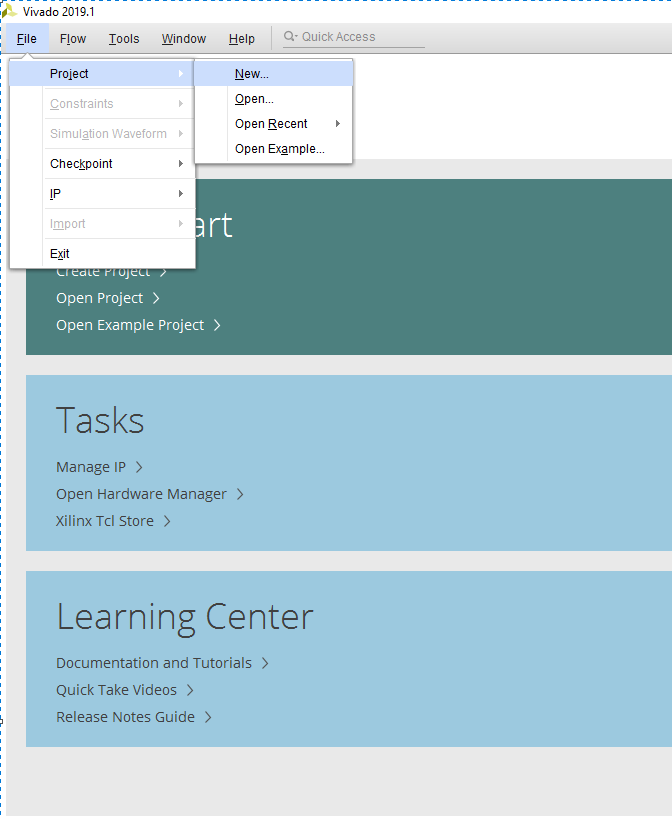
\includegraphics[width=0.3\textwidth]{image/m_3.png}
	\caption{Создание нового проекта в Vivado}
	\label{l1_new_prj}
\end{figure}

\begin{figure}[!ht]
	\centering
	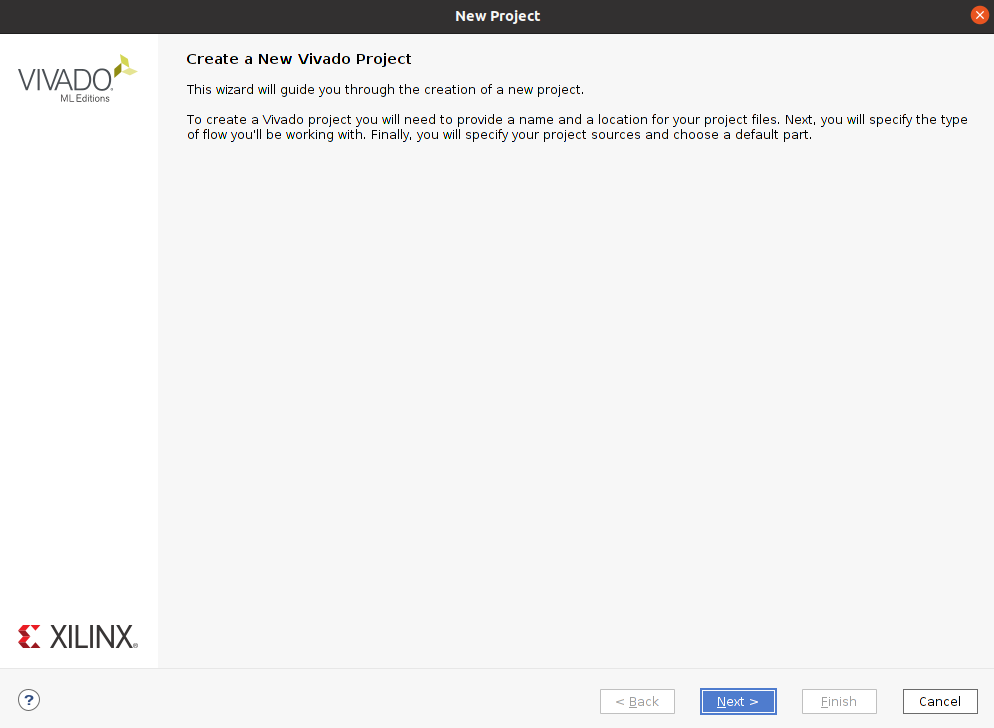
\includegraphics[width=0.4\textwidth]{image/2}
	\caption{Окно мастера создания нового проекта}
	\label{l1_master}
\end{figure}

Для создания проекта щелкните «File->Project->New» на панели быстрого запуска, как показано на рисунке ~\ref{l1_new_prj}. Откроется диалоговое окно «New project», как показано на рисунке ~\ref{l1_master}. Нажмите «Next», чтобы продолжить.

\newpage

\begin{figure}[!ht]
	\centering
	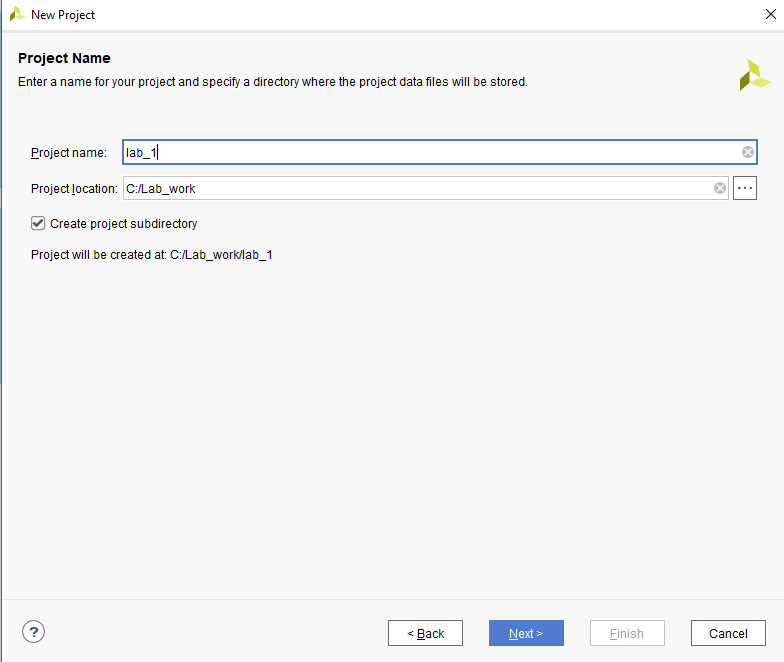
\includegraphics[width=0.4\textwidth]{image/l1_lab_1}
	\caption{Название проекта, путь к проекту}
	\label{l1_name}
\end{figure}
Введите название проекта, как показано на рисунке~\ref{l1_name}. Обычно рекомендуется сделать название проекта более информативным, чтобы вам было легче идентифицировать свои проекты в будущем. Например, если вы разрабатываете семисегментный контроллер, вы можете назвать проект «Семисегментный контроллер». Вам следует избегать использования пробелов в имени или расположении проекта, потому что пробелы могут привести к сбою некоторых инструментов.

\begin{figure}[!ht]
	\centering
	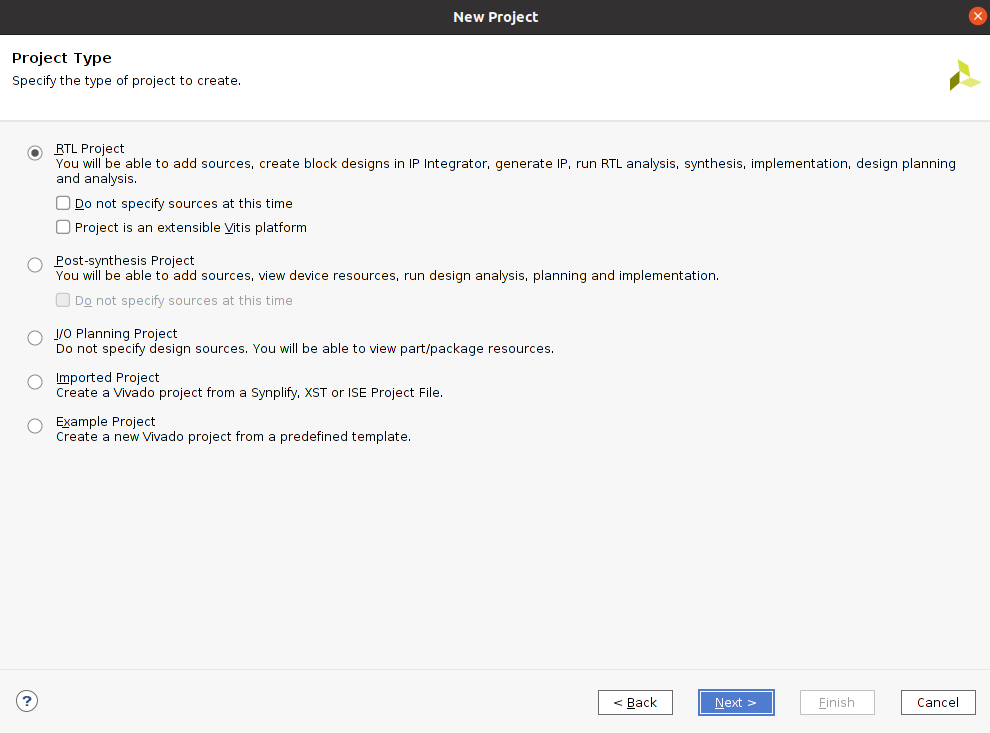
\includegraphics[width=0.4\textwidth]{image/8}
	\caption{Выбор типа создаваемого  проекта}
	\label{l1_type_prj}
\end{figure}

«Project Type» настраивает определенные инструменты дизайна и внешний вид IDE в зависимости от типа проекта, который вы собираетесь создать. В большинстве случаев вы выбираете «RTL Project»,чтобы настроить инструменты для создания нового дизайна, как показано на рисунке ~\ref{l1_type_prj}.

\begin{figure}[!ht]
	\centering
	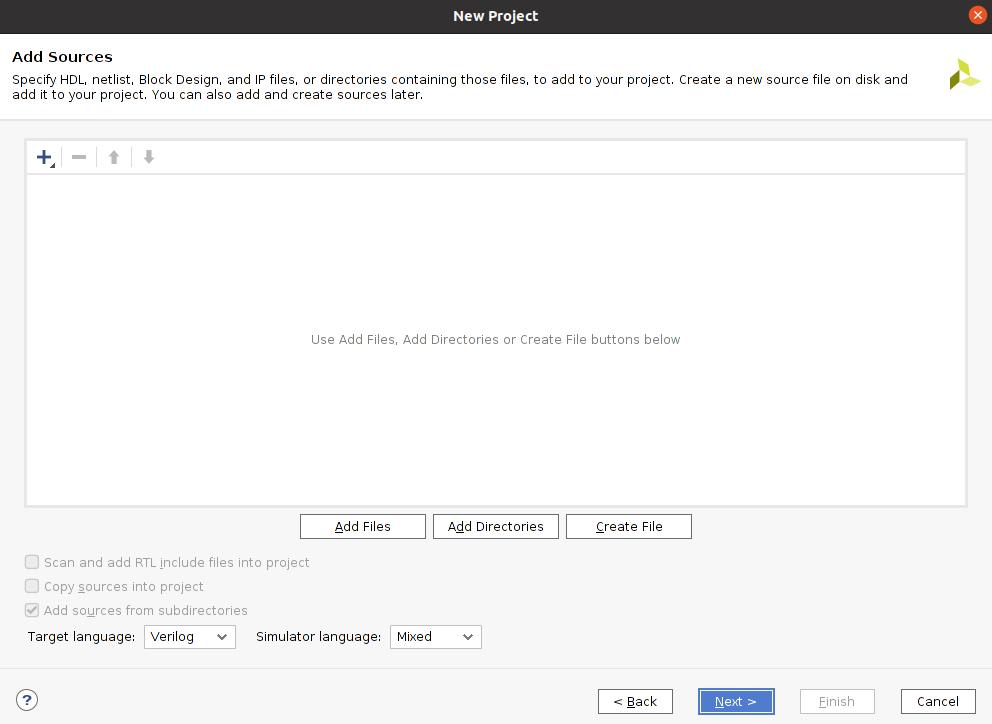
\includegraphics[width=0.4\textwidth]{image/9}
	\caption{Подключение исходных файлов}
	\label{l1_source}
\end{figure}

В новом дизайне вы не добавляете какие-либо существующие источники, потому что вы их еще не создали.

На данный момент нет существующих источников для добавления, поэтому просто нажмите «Next» (см. рис. ~\ref{l1_source}).

\begin{figure}[!ht]
	\centering
	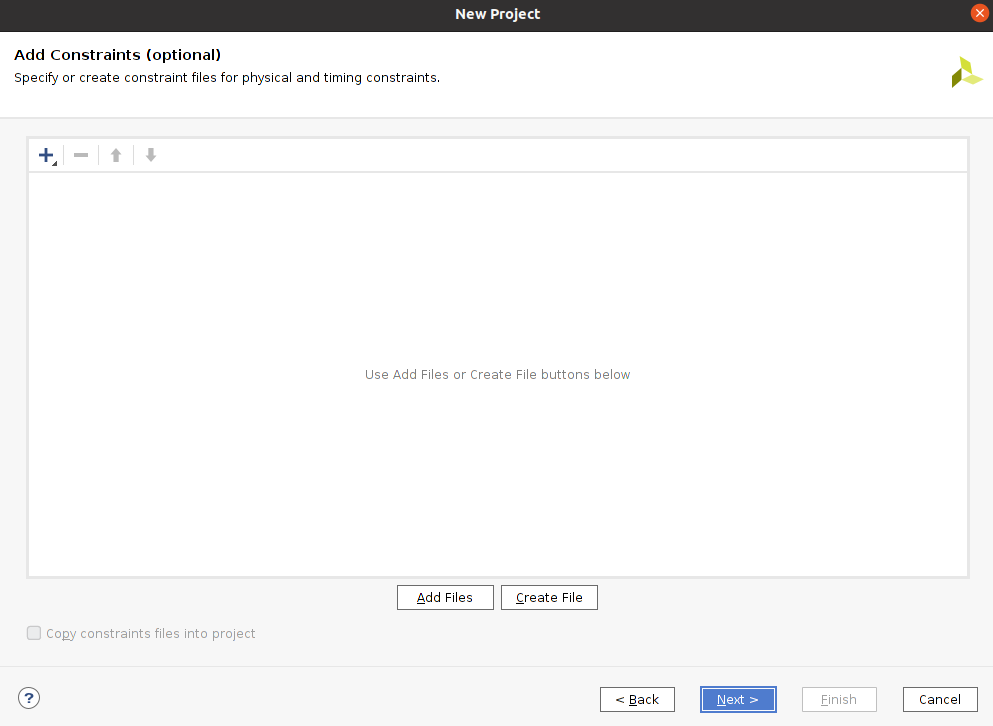
\includegraphics[width=0.4\textwidth]{image/10}
	\caption{Подключение .xdc файлов}
	\label{l1_xdc}
\end{figure}

Файлы ограничений предоставляют информацию о физической реализации проекта. 

Позже в этом руководстве вы создадите файл ограничений, чтобы определить, какие именованные узлы схемы должны быть подключены к каким физическим контактам. Но на данный момент у вас нет существующего файла ограничений для добавления, поэтому вы можете просто нажать «Next»(см. рис. ~\ref{l1_xdc}).

\begin{figure}[!ht]
	\centering
	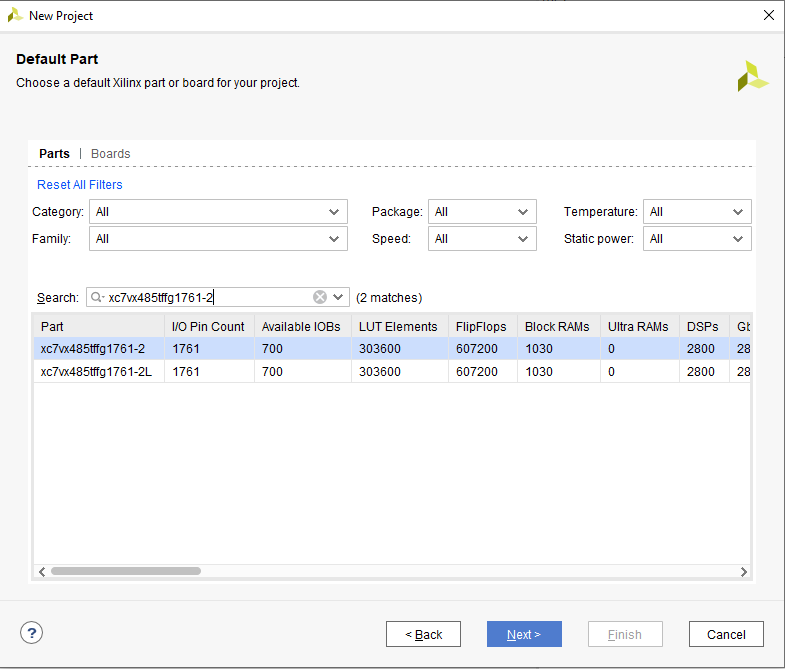
\includegraphics[width=0.4\textwidth]{image/m_9.png}
	\caption{Выбор FPGA}
	\label{l1_fpga}
\end{figure}

Xilinx производит множество различных ПЛИС, и синтезатору необходимо точно знать, какую вы используете, чтобы он мог создать корректную прошивку. На отладочной плате VC707 установлена \verb|xc7vx485tffg1761-2|. Выберете ПЛИС, как показано на рисунке ~\ref{l1_fpga}.

\begin{figure}[!ht]
	\centering
	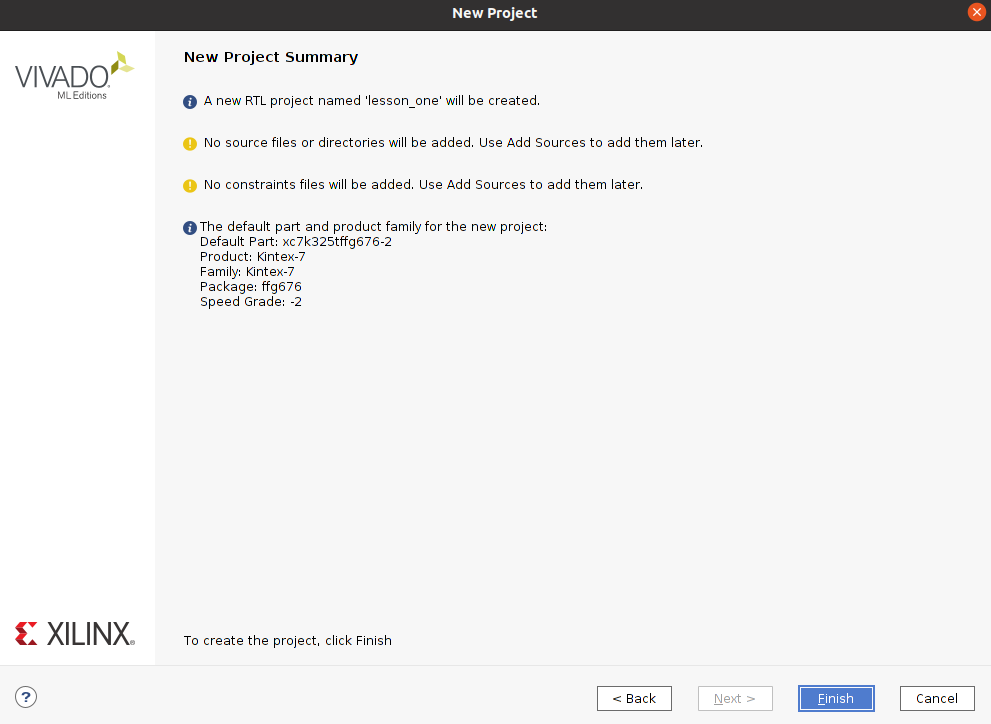
\includegraphics[width=0.4\textwidth]{image/summary}
	\caption{Cуммарные сведения о создаваемом проекте}
	\label{l1_sum}
\end{figure}

На последней странице мастера создания проекта отображается сводка конфигурации проекта. Убедитесь, что вся информация в сводке верна, и, в частности, убедитесь, что выбрана правильная часть FPGA. Если что-то не так, нажмите назад и исправьте; в противном случае нажмите Готово, чтобы завершить создание пустого проекта. Cуммарные сведения о создаваемом проекте представлены на рисунке ~\ref{l1_sum}.

\subsection{Шаг 2: создаём исходные файлы проекта}

\begin{figure}[htbp]	
	\subfigure[Схема подключения светодиодов к ПЛИС] 
	{
		\begin{minipage}{8cm}
			\centering         
			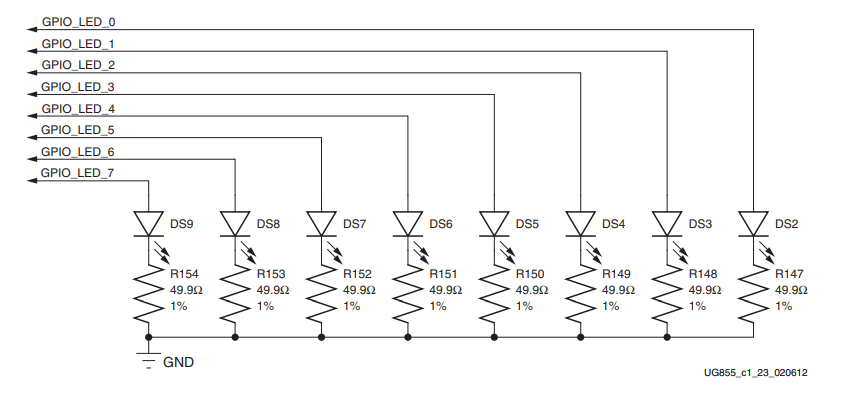
\includegraphics[scale=0.4]{image/LEDS.png}
			\label{LEDS}
		\end{minipage}
	}
	\subfigure[Схема подключения кнопок к ПЛИС] 
	{
		\begin{minipage}{8cm}
			\centering      
			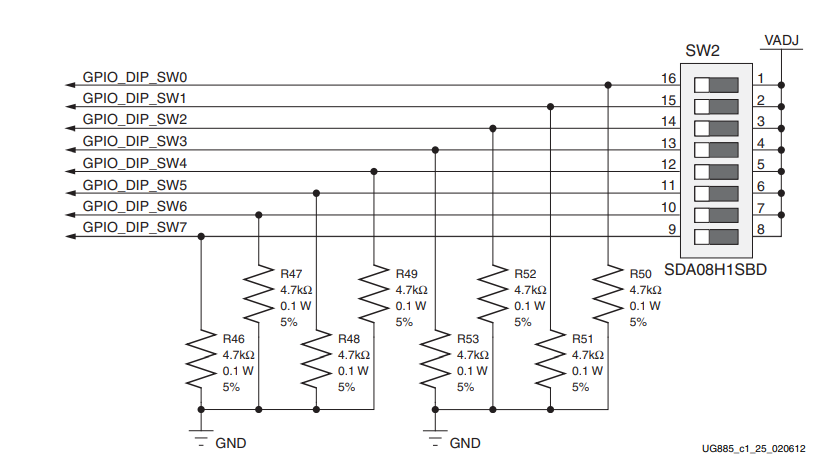
\includegraphics[scale=0.4]{image/DIP_SWITCH.png}
			\label{DIP_SWITCH}
		\end{minipage}
	}
	\caption{Схемы подключения светодиодов и кнопок к ПЛИС} %  %Имя большого изображения
\end{figure}

\begin{figure}[!ht]
	\centering
	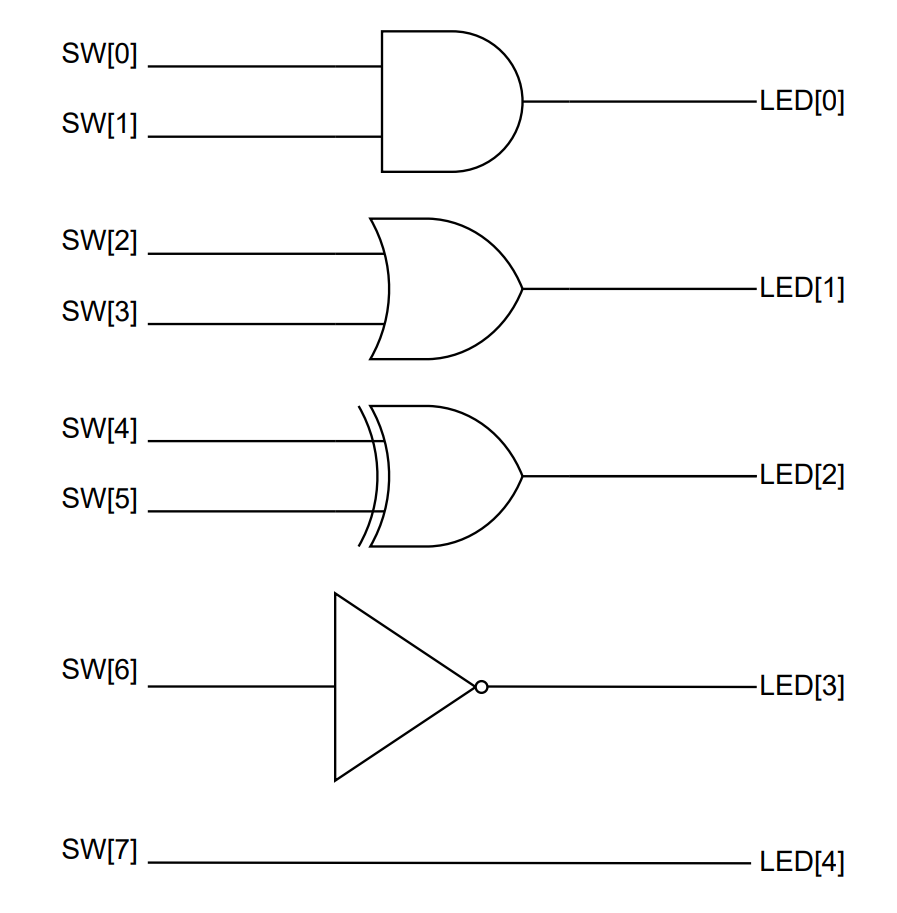
\includegraphics[width=0.3\textwidth]{image/module_0.png}
	\caption{Схема реализуемого модуля}
	\label{module_0}
\end{figure}

Для всех проектов требуются как минимум два типа исходных файлов - файл HDL (Verilog или VHDL) для описания схемы и файл ограничений, чтобы предоставить синтезатору информацию, необходимую для сопоставления вашей схемы с целевой микросхемой.

После создания исходного файла Verilog его можно смоделировать напрямую. Моделирование (более подробно обсуждается позже) позволяет вам работать с компьютерной моделью схемы, поэтому вы можете проверить ее поведение, прежде чем тратить время на ее реализацию на физическом устройстве. Симулятор позволяет вам управлять всеми входами схемы с различными шаблонами с течением времени и проверять, что выходы ведут себя должным образом во всех условиях.

В первой лаборатоной работе вам предоставлены исходные Verilog файл и файл ограничений. Вместо того, чтобы создавать их самостоятельно, как это обычно бывает, вы можете просто скопировать их в пустые исходные файлы или загрузить напрямую в свой проект. В более поздних проектах вы создадите эти файлы самостоятельно.

В данной лабораторной работе будет реализован простейший проект подключения кнопок к светодиодам через логические вентили. Схема электрическая принципиальная подключения светодиодов и кнопок представлены соотвественно на рисунках ~\ref{LEDS}, ~\ref{DIP_SWITCH}. Схема реализуемого модуля представлена на рисунке ~\ref{module_0}.

\subsubsection{Создание HDL-файлов}

\begin{figure}[htbp]	
	\subfigure[Add sources] 
	{
		\begin{minipage}{8cm}
			\centering         
			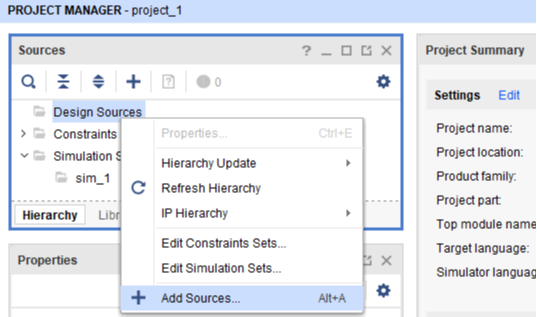
\includegraphics[scale=0.4]{image/l_1_sources.png}   
			\label{add_source_0}
		\end{minipage}
	}
	\subfigure[Окно мастера подключения нового файла] 
	{
		\begin{minipage}{8cm}
			\centering      
			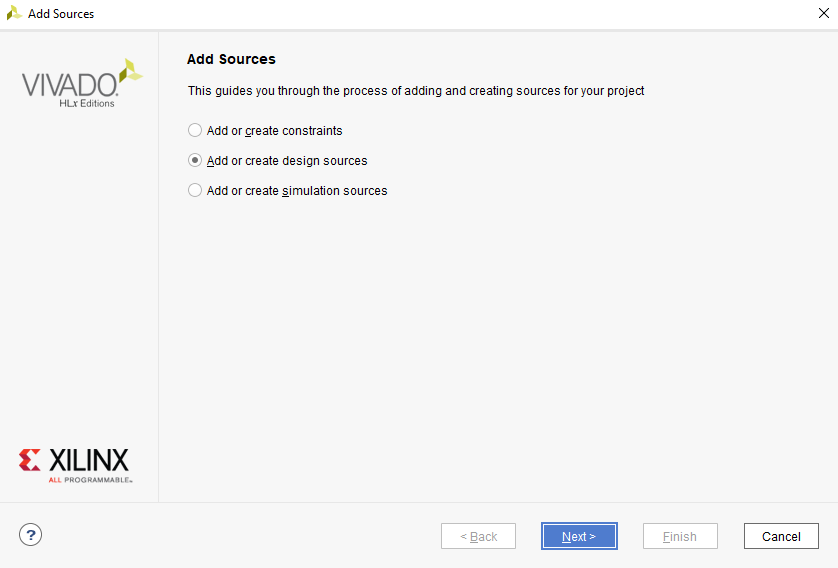
\includegraphics[scale=0.3]{image/l_2_sources.png}   
			\label{add_source_1}
		\end{minipage}
	}
	\caption{Окно мастера подключения нового файла: внешний вид} %  %Имя большого изображения
\end{figure}


\begin{figure}[htbp]	
	\subfigure[Назначаем файлу имя] 
	{
		\begin{minipage}{8cm}
			\centering         
			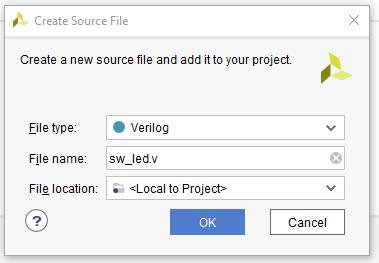
\includegraphics[scale=0.6]{image/sw_led.png}   
			\label{add_source_2}
		\end{minipage}
	}
	\subfigure[Результаты добавления файла] 
	{
		\begin{minipage}{8cm}
			\centering      
			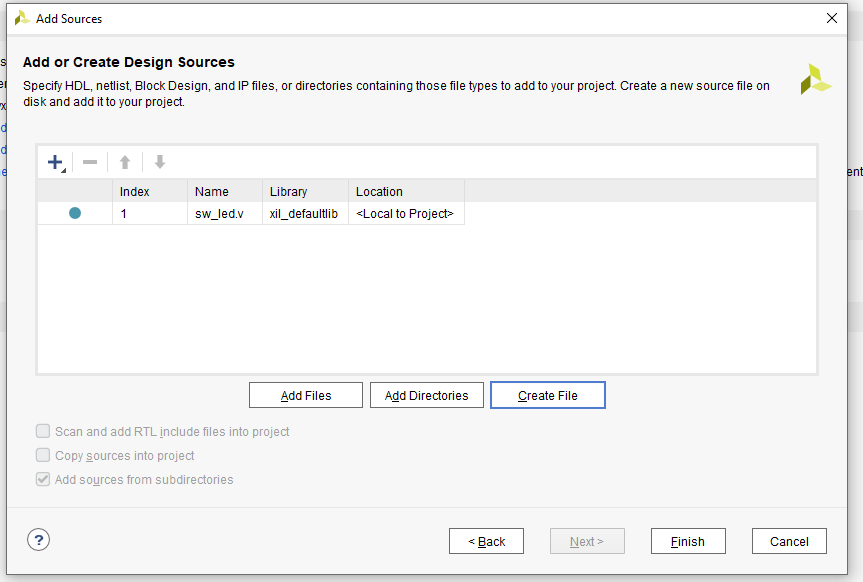
\includegraphics[scale=0.4]{image/sw_led_2.png}   
			\label{add_source_3}
		\end{minipage}
	}
	\caption{Окно мастера подключения нового файла: имя и результаты} %  %Имя большого изображения
\end{figure}

Чтобы создать исходный файл Verilog для вашего проекта, щелкните правой кнопкой мыши «Design Sources» на панели «Sources» и выберите «Add sources»(см. рис. ~\ref{add_source_0}). Появится диалоговое окно «Add sources», как показано на рисунке ~\ref{add_source_1} - выберите «Add or create design sources» и нажмите «Далее».

В диалоговом окне «Add or Create Design Sources» нажмите «Create File», введите имя файла \verb|sw_led| и нажмите «ОК»(см. рис. ~\ref{add_source_2},~\ref{add_source_3}). Вновь созданный файл появится в списке, как показано на рисунке. Нажмите Finish, чтобы перейти к следующему шагу.

Откроется диалоговое окно «define module» и представляет собой область, в которой вы можете определить входные и выходные порты для вашей схемы. В более поздних проектах, если вы введете здесь имена портов, Vivado создаст исходный файл Verilog с уже определенными портами. Для этого упражнения предоставляется полный исходный файл, поэтому вы можете пропустить этот шаг, нажав OK (а затем YES), чтобы продолжить.

Теперь вы увидите, что \verb|sw_led| указан в папке «Design Sources» на панели «Sources». Дважды щелкните \verb|sw_led|, чтобы открыть файл, и замените содержимое (скопируйте и вставьте) приведенным ниже кодом.

\begin{Verbatim}[tabsize=4]
`timescale 1ns / 1ps

module sw_led(
    input wire [7:0] sw,
    output wire [7:0] led
);

    assign led[0] = sw[0] & sw[1];
    assign led[1] = sw[2] | sw[3];
    assign led[2] = sw[4] ^ sw[5];
    assign led[3] = ~sw[6];
    assign led[4] = sw[7];
    assign led[5] = 1'b0;
    assign led[6] = 1'b1;
    assign led[7] = 1'b0;
    
endmodule
\end{Verbatim}

Начнём рассмотрение языка Verilog. Основой описания на Verilog явяляется модуль, представляемый в виде отдельного файла с расширенией .v. 
Структура модуля на языке Verilog имеет следующий вид:

\begin{Verbatim}[tabsize=4]
`timescale 1ns/1ps

module <имя> #(
	[параметры]
)
(
	<объявление портов>
);
[объявление локальных сигналов и переменных]
<синтезируемые конструкции>
endmodule

\end{Verbatim}

Существует три типа портов: вход(input), выход(output), двунаправленный вывод(inout).

Директива `'timescale предназначена для задания временных интервалов моделирования. Первый из них задаёт длительность единицы времени по умолчанию для моделирования.
Второй параметр задаёт величину дискретного шага, используемого средствами моделирования.

Рассмотри реализацию данного модуля. Он соединяет восемь переключателей со светодиодами через логические вентили И, ИЛИ, Исключающее ИЛИ, НЕ. 
Тип порта кнопок объявлен как входной(input), а светодиодов выходной(output). При этом заметим, что порты содержат не один провод, а целую шину - множество проводов, в данном случае по восемь штук. Используя оператор непрерывного присваивания \verb|assign| подключаем кнопки к светодиодам через логические вентили. На оставшиеся светодиоды \verb|led[5], led[6], led[7]| подключим логический ноль, логическую единицу, логический ноль соответственно.

Рассмотрим подробнее синтаксис и свойства оператора непрерывного назначения \verb|assign|.  Синтаксис имеет следующий вид:

\begin{Verbatim}[tabsize=4]
assign #(delay) net_name = expression;
\end{Verbatim}

Оператор непрерывного назначения \verb|assign| функционирует следующим образом. При любом изменении любого из значений в выражении expression с правой стороны, заново вычисляется выражение 
expression и полученное значение по истечении времени, определяемого задержкой delay, присваивается величине слева от знака =.

\subsubsection{Создание файлов ограничений}

\begin{figure}[htbp]	
	\subfigure[Назначаем файлу ограничений имя] 
	{
		\begin{minipage}{8cm}
			\centering         
			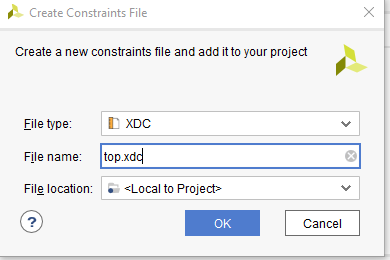
\includegraphics[scale=0.6]{image/xdc.png}   
			\label{add_xdc}
		\end{minipage}
	}
	\subfigure[Результаты добавления файла ограничений] 
	{
		\begin{minipage}{8cm}
			\centering      
			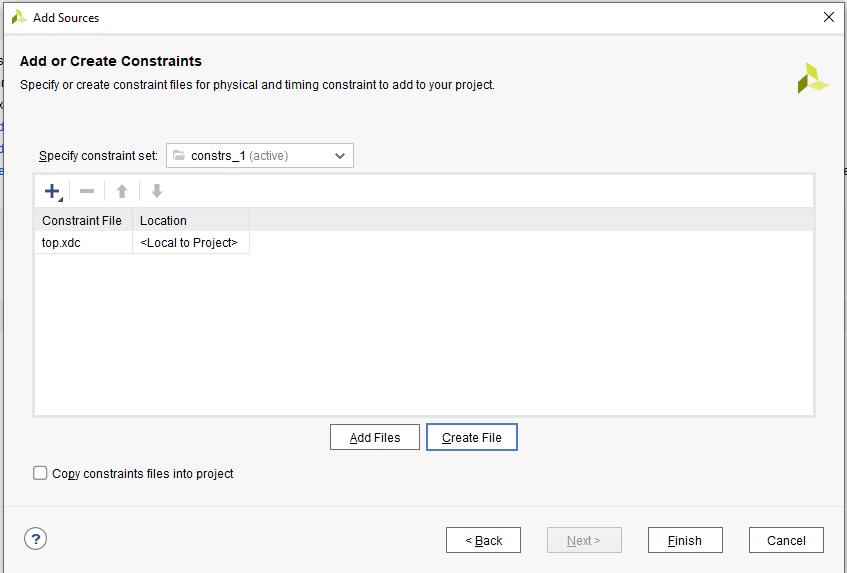
\includegraphics[scale=0.4]{image/xdc_2.png}   
			\label{add_xdc_0}
		\end{minipage}
	}
	\caption{Окно мастера подключения нового файла: имя и результаты} %  %Имя большого изображения
\end{figure}{}

\begin{figure}[!ht]
	\centering
	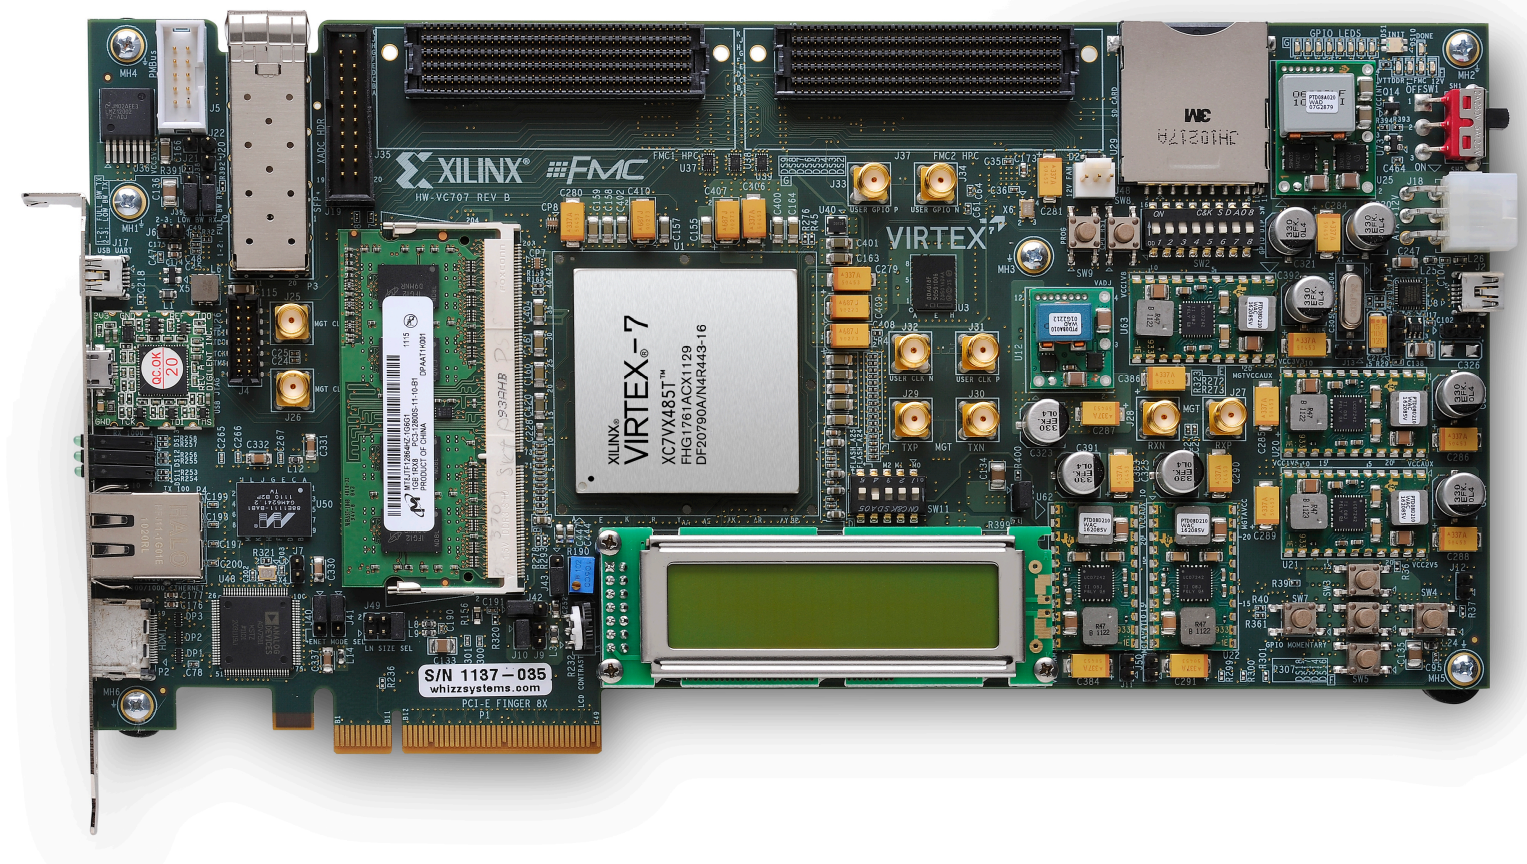
\includegraphics[width=0.4\textwidth]{image/VC707.png}
	\caption{Внешний вид отладочной платы VC707}
	\label{VC707}
\end{figure}

Исходные файлы Verilog описывают только поведение схемы. Вы также должны предоставить файл ограничений, чтобы сопоставить ваш дизайн с физическим чипом и платой, с которыми вы работаете.
В файле ограничений указывается к какому физическому выводу ПЛИС подключечается данный вывод нашего Verilog модуля, а также электрический стандарт используемый для вывода.

Для того чтобы определить, к каким выводам ПЛИС подключать сигналы, недостаточно информации, имеющейся в САПР или в документации на саму ПЛИС. После установки ПЛИС на плату внешние компоненты могут быть подключены производятелем платы самыми разными способами, поэтому требуется обратиться к технической документации на печатную плату. Для проекта была выбрана плата VC707 производства компании Xilinx, на которой и установлена ПЛИС Virtex-7, заданная в настройках проекта. Внешний вид платы представлен на рисунке ~\ref{VC707}. Обратившись к технической документации, можно найти следующую информацию:

\begin{enumerate}
	\item AM39, AN39, AR37, AT37, AR35, AP41, AP42, AU39 - выходы ПЛИС подключенные к светодиодам(\verb|GPIO_LED_0|, \verb|GPIO_LED_1| и т.д (см.рис. ~\ref{LEDS}));
	\item AV30, AY33, BA31, BA32, AW30, AY30, BA30, BB31 - входы ПЛИС подключенные к переключателям платы(\verb|GPIO_DIP_SW_0|, \verb|GPIO_DIP_SW_1| и т.д (см.рис. ~\ref{DIP_SWITCH})).
\end{enumerate}

Также для формата xdc обязательным требованием является явное указание электрического стандарта, используемого для вывода. 

По этому поводу необходимо сделать важное пояснение. ПЛИС не имеют возможности подключать заданные разработчиком напряжения к буферам ввода-вывода, ориентируясь на заданные в файле xdc 
сведения. Для питания будут использованы напряжения, фактически поданные на банки ввода-вывода. Неверное указание напряжения в файле xdc не приведет к выходу ПЛИС из строя, однако рассчи- задержки распространения сигналов окажутся неверными ( они зависят от используемого напряжения питания). Однако для всех выводов, находящихся в одном банке ввода-вывода, требуется, чтобы напряжение электрических интерфейсов было одним и тем. Потому разработчик должен явно указать в файле проектных ограничений электрический интерфейс, который он рассчитывает использовать При появлении в одном банке интерфейсов с разным напряжением САПР сгенерирует ошибку и создание конфигурациного файла будет запрещено. 

Рассмотрим пример:

\begin{Verbatim}[tabsize=4]
set_property PACKAGE_PIN AM39 [get_ports {led[0]}]
set_property IOSTANDARD LVCMOS18 [get_ports {led[0]}]
\end{Verbatim}

Первая строка подключает вывод \verb|led[0]| к контакту AM39 ПЛИС. Вторая строка задаёт  электрический стандарт LVCMOS18 для этого вывода.

Чтобы создать файл ограничений, разверните заголовок «Constraints» на панели «Sources», щелкните правой кнопкой мыши \verb|constrs_1| и выберите «Add Sources» (или, что то же самое, нажмите «Add Sources» в окне «Flow Navigator» в «Project Manager»)(см. рис. ~\ref{add_xdc}, ~\ref{add_xdc_0}) .

Появится диалоговое окно «Add Sources». Выберите «Add or Create Constraints» и нажмите «Далее», чтобы открыть диалоговое окно «Add or Create Constraints».

Нажмите «Create File», введите имя файла «top» и нажмите «ОК». Вновь созданный файл появится в списке, как показано на рисунке. Нажмите Готово, чтобы перейти к следующему шагу.

\begin{Verbatim}[tabsize=4]
# LEDs
set_property PACKAGE_PIN AM39 [get_ports {led[0]}]
set_property IOSTANDARD LVCMOS18 [get_ports {led[0]}]
set_property PACKAGE_PIN AN39 [get_ports {led[1]}]
set_property IOSTANDARD LVCMOS18 [get_ports {led[1]}]
set_property PACKAGE_PIN AR37 [get_ports {led[2]}]
set_property IOSTANDARD LVCMOS18 [get_ports {led[2]}]
set_property PACKAGE_PIN AT37 [get_ports {led[3]}]
set_property IOSTANDARD LVCMOS18 [get_ports {led[3]}]
set_property PACKAGE_PIN AR35 [get_ports {led[4]}]
set_property IOSTANDARD LVCMOS18 [get_ports {led[4]}]
set_property PACKAGE_PIN AP41 [get_ports {led[5]}]
set_property IOSTANDARD LVCMOS18 [get_ports {led[5]}]
set_property PACKAGE_PIN AP42 [get_ports {led[6]}]
set_property IOSTANDARD LVCMOS18 [get_ports {led[6]}]
set_property PACKAGE_PIN AU39 [get_ports {led[7]}]
set_property IOSTANDARD LVCMOS18 [get_ports {led[7]}]

# DIP Switches
set_property PACKAGE_PIN AV30 [get_ports {sw[0]}]
set_property IOSTANDARD LVCMOS18 [get_ports {sw[0]}]
set_property PACKAGE_PIN AY33 [get_ports {sw[1]}]
set_property IOSTANDARD LVCMOS18 [get_ports {sw[1]}]
set_property PACKAGE_PIN BA31 [get_ports {sw[2]}]
set_property IOSTANDARD LVCMOS18 [get_ports {sw[2]}]
set_property PACKAGE_PIN BA32 [get_ports {sw[3]}]
set_property IOSTANDARD LVCMOS18 [get_ports {sw[3]}]
set_property PACKAGE_PIN AW30 [get_ports {sw[4]}]
set_property IOSTANDARD LVCMOS18 [get_ports {sw[4]}]
set_property PACKAGE_PIN AY30 [get_ports {sw[5]}]
set_property IOSTANDARD LVCMOS18 [get_ports {sw[5]}]
set_property PACKAGE_PIN BA30 [get_ports {sw[6]}]
set_property IOSTANDARD LVCMOS18 [get_ports {sw[6]}]
set_property PACKAGE_PIN BB31 [get_ports {sw[7]}]
set_property IOSTANDARD LVCMOS18 [get_ports {sw[7]}]
\end{Verbatim}

Теперь вы увидите файл \verb|top.xdc| в списке под папкой \verb|Constraints/constrs_1| на панели «SourcesИ». Дважды щелкните \verb|top.xdc|, чтобы открыть файл, и замените содержимое приведенным ниже кодом.

\subsubsection{Основы моделирования в Vivado}

Чтобы создать исходный файл моделирования для вашего проекта, щелкните правой кнопкой мыши «Simulation Sources» на панели «Sources» и выберите «Add sources». Появится диалоговое окно «Add sources», как показано - выберите «Add or create simulation sources» и нажмите «Next». На рисунках ниже представлен подробный алгоритм добавления нового файла верификации.

В диалоговом окне «Add or create simulation sources» нажмите «Create File», введите имя файла \verb|tb_sw_led.v| и нажмите «ОК». Вновь созданный файл появится в списке, как показано на рисунке. Нажмите Finish, чтобы перейти к следующему шагу. Теперь вы увидите, что \verb|tb_sw_led.v| указан в папке «Simulation Sources» на панели «Sources». 

Дважды щелкните \verb|tb_sw_led.v|, чтобы открыть файл, и замените содержимое (скопируйте и вставьте) приведенным ниже кодом.

\begin{figure}[htbp]	
	\subfigure[Add or create simulation source] 
	{
		\begin{minipage}{8cm}
			\centering         
			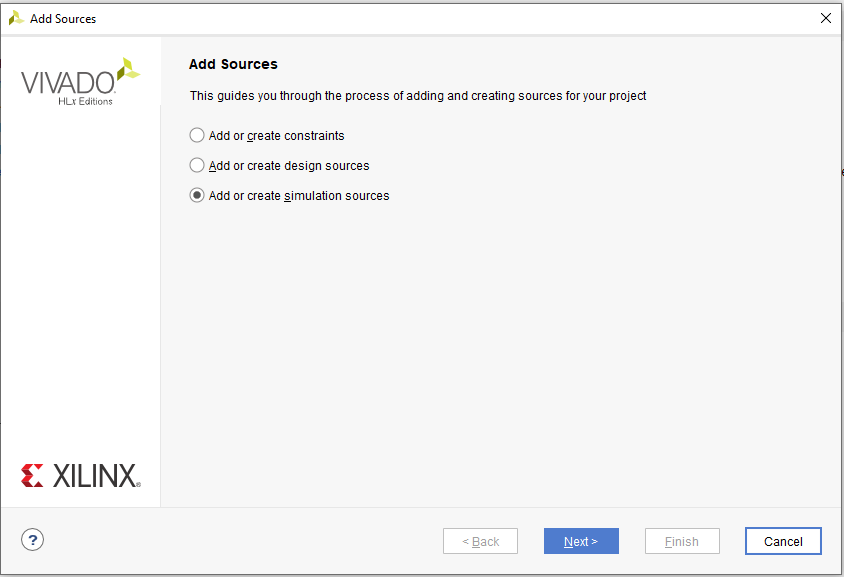
\includegraphics[scale=0.3]{image/l1_sim_1.png}   
			\label{Start_V}
		\end{minipage}
	}
	\subfigure[Окно мастера подключения нового файла] 
	{
		\begin{minipage}{8cm}
			\centering      
			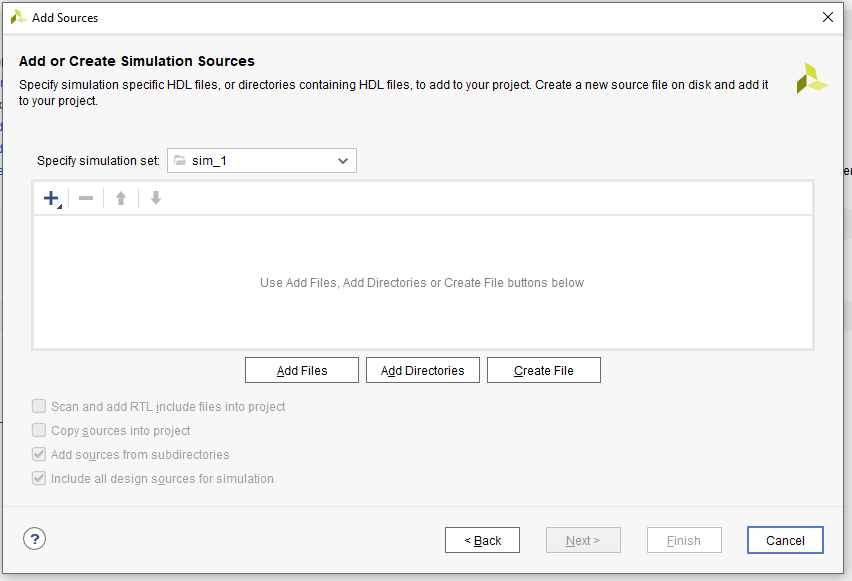
\includegraphics[scale=0.3]{image/l1_sim_2.png}   
			\label{Win_Project}
		\end{minipage}
	}
	\caption{Окно мастера подключения нового файла: внешний вид} %  %Имя большого изображения
\end{figure}

\begin{figure}[htbp]	
	\subfigure[Назначаем файлу моделирования имя] 
	{
		\begin{minipage}{8cm}
			\centering         
			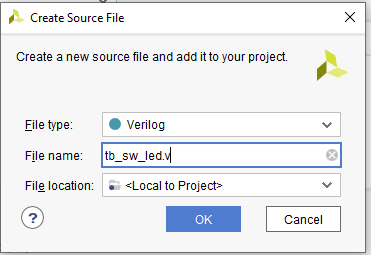
\includegraphics[scale=0.7]{image/l1_sim_3.png}   
			\label{Start_V}
		\end{minipage}
	}
	\subfigure[Результаты добавления файла моделирования] 
	{
		\begin{minipage}{8cm}
			\centering      
			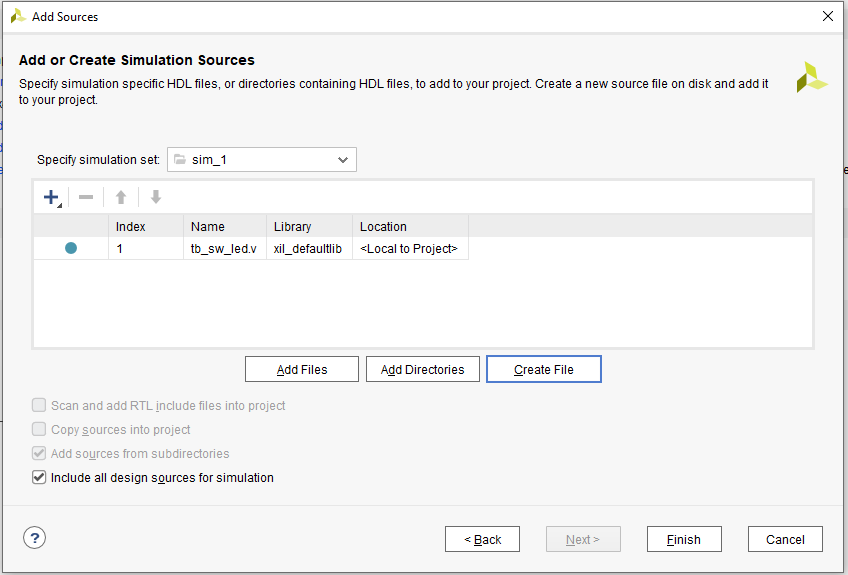
\includegraphics[scale=0.4]{image/l1_sim_4.png}   
			\label{Win_Project}
		\end{minipage}
	}
	\caption{Окно мастера подключения нового файла: имя и результаты} %  %Имя большого изображения
\end{figure}

\begin{Verbatim}[tabsize=4]
`timescale 1ns / 1ps
module tb_sw_led();
    
reg [7:0] sw_led_reg;
wire [7:0] led_w;

sw_led
sw_led_inst
(
    .sw(sw_led_reg),
    .led(led_w)
);

initial begin
    $display("Result:",);
    $timeformat(-9,1,"ns",8);
    $monitor($time, 
    	": 	sw[0] & sw[1]= %b; 
    		sw[2] | sw[3]=%b; 
    		sw[4] ^ sw[5]=%b; 
    		~sw[6]=%b; 
    		sw[7] = %b;", 
    		led_w[0],
    		led_w[1], 
    		led_w[2], 
    		led_w[3], 
    		led_w[4]);
    sw_led_reg[0] = 0;
    sw_led_reg[1] = 0;
    sw_led_reg[2] = 0;
    sw_led_reg[3] = 0;
    sw_led_reg[4] = 0;
    sw_led_reg[5] = 0;
    sw_led_reg[6] = 0;
    sw_led_reg[7] = 0;
    #100;
    sw_led_reg[0] = 0;
    sw_led_reg[1] = 1;
    sw_led_reg[2] = 0;
    sw_led_reg[3] = 1;
    sw_led_reg[4] = 0;
    sw_led_reg[5] = 1;
    sw_led_reg[6] = 0;
    sw_led_reg[7] = 1;
    #100;
    sw_led_reg[0] = 1;
    sw_led_reg[1] = 0;
    sw_led_reg[2] = 1;
    sw_led_reg[3] = 0;
    sw_led_reg[4] = 1;
    sw_led_reg[5] = 0;
    sw_led_reg[6] = 1;
    sw_led_reg[7] = 0;
    #100;
    sw_led_reg[0] = 1;
    sw_led_reg[1] = 1;
    sw_led_reg[2] = 1;
    sw_led_reg[3] = 1;
    sw_led_reg[4] = 1;
    sw_led_reg[5] = 1;
    sw_led_reg[6] = 1;
    sw_led_reg[7] = 1;
end

endmodule
\end{Verbatim}

\begin{figure}[!ht]
	\centering
	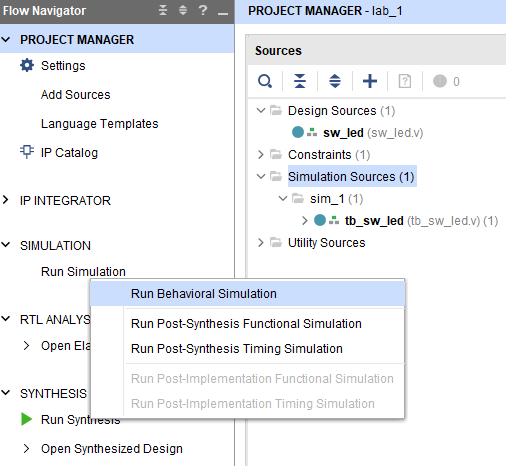
\includegraphics[width=0.4\textwidth]{image/sim_rub.png}
	\caption{Запуск симуляции в среде Vivado}
	\label{prj_sum}
\end{figure}

\begin{figure}[!ht]
	\centering
	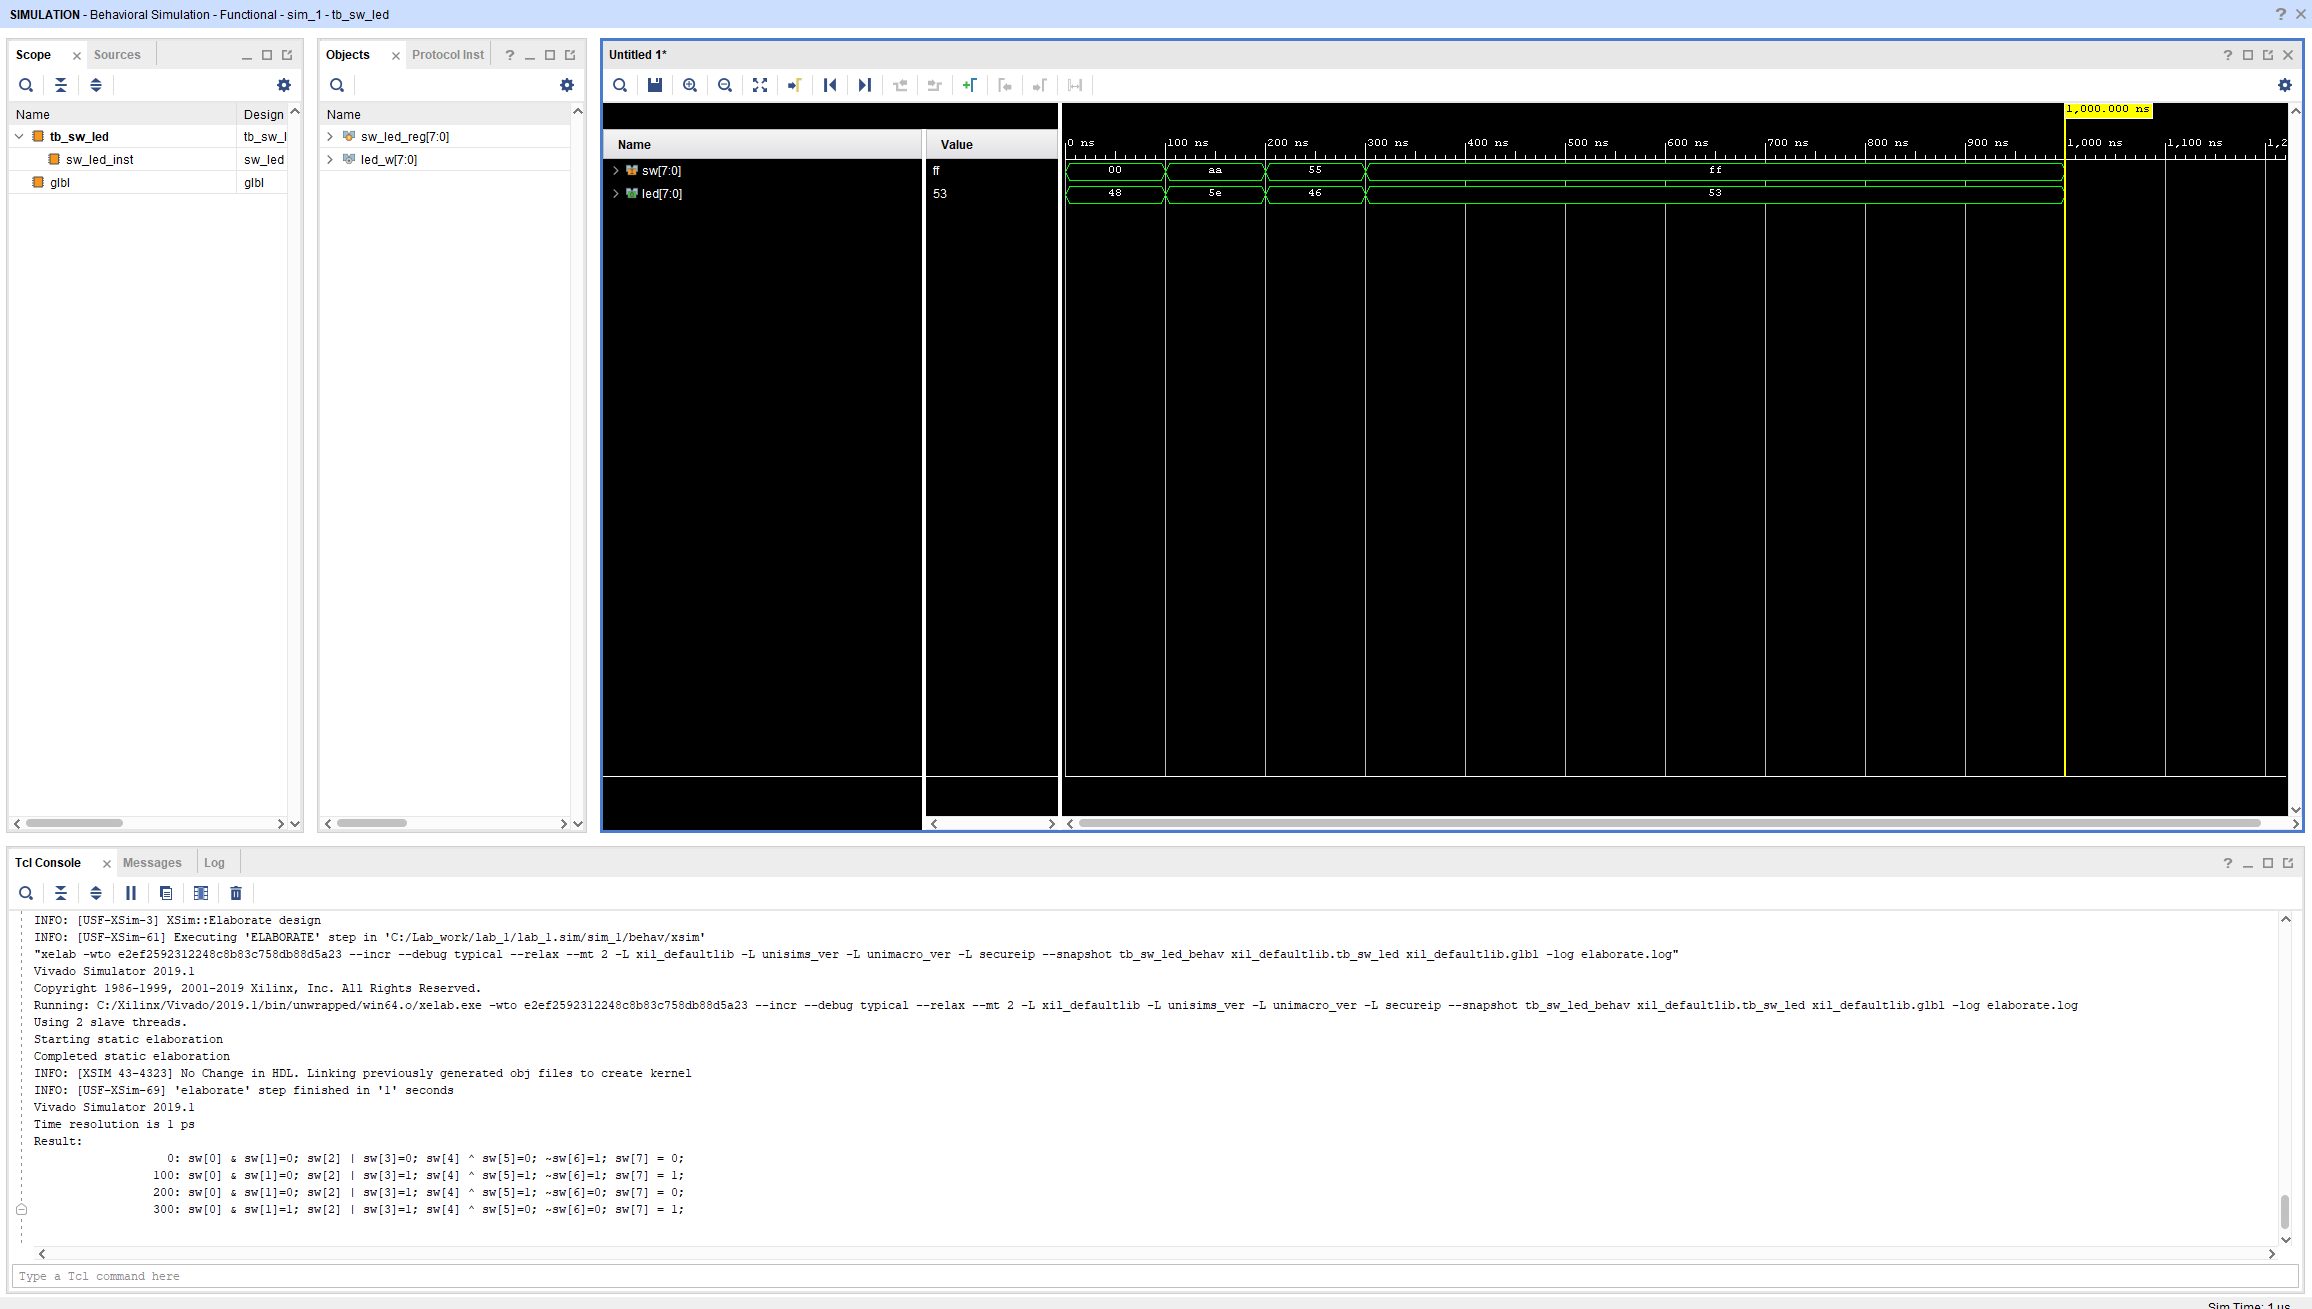
\includegraphics[width=0.7\textwidth]{image/l1_sim_5.png}
	\caption{Окно симуляции в среде Vivado}
	\label{prj_sum}
\end{figure}

Для запуска моделирования нажмите Run Simulation на панели Flow Navigator.
Результат симуляции схемы.

\begin{Verbatim}[tabsize=4]
Result: 

0: sw[0] & sw[1]=0; sw[2] | sw[3]=0; sw[4] ^ sw[5]=0;~sw[6]=1;sw[7] = 0;
100: sw[0] & sw[1]=0; sw[2] | sw[3]=1; sw[4] ^ sw[5]=1;~sw[6]=1;sw[7] = 1;
200: sw[0] & sw[1]=0; sw[2] | sw[3]=1; sw[4] ^ sw[5]=1;~sw[6]=0;sw[7] = 0;
300: sw[0] & sw[1]=1; sw[2] | sw[3]=1; sw[4] ^ sw[5]=0;~sw[6]=0;sw[7] = 1;
\end{Verbatim}
\subsection{Шаг 3: Synthesis, Implementation, and Generate Bitstream}

\subsubsection{Синтез}

После того, как ваши файлы Verilog и файлы ограничений будут завершены, вы можете синтезировать проект. В процессе синтеза код Verilog преобразуется в «список соединений», который определяет все необходимые компоненты схемы(эти компоненты являются программируемыми частями целевого логического устройства). Вы можете запустить процесс синтеза, нажав кнопку «Run Synthesis» на панели «Flow Navigator», как показано на рисунке.

Примечание. В конце процесса синтеза открывается диалоговое окно с вопросом, что вы хотите делать дальше. Это просто удобство — он показывает те же варианты, что и в окне Flow Navigator. Вы можете просто закрыть окно или выбрать «Implement Design», который является следующим шагом (см. ниже).

\begin{figure}[!ht]
	\centering
	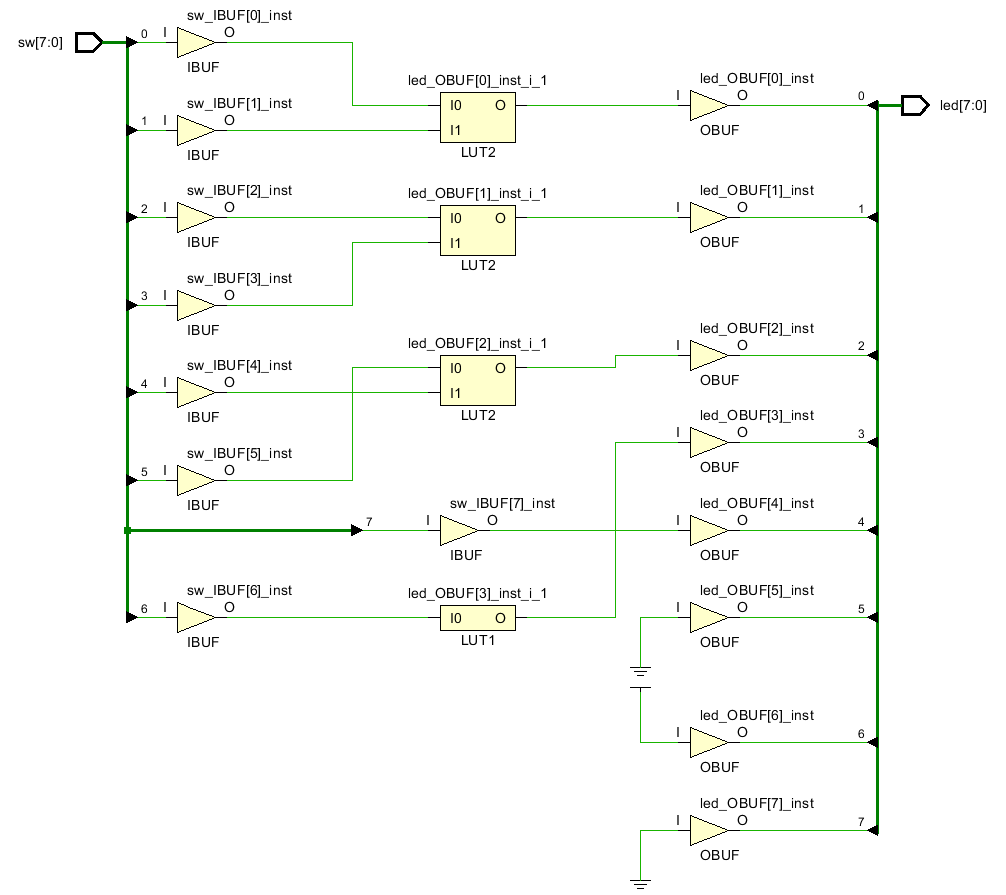
\includegraphics[width=0.7\textwidth]{image/synth.PNG}
	\caption{Синтезированный дизайн}
	\label{l1_synth}
\end{figure}

\subsubsection{Размещение и трассировка проекта}

Эта группа проектных действий входит в состав стадии САПР implementation, название которой дословно можно перевести как «реализация» или сосуществление», однако в русском языке этот термин является не сколько неопределенным и его трудно однозначно связать с проектным шагом, а не просто с общим процессом работы над проектом. 
На данной стадии производится преобразование списка связей в информацию о размещении отдельных элементов ПЛИС на кристалле и настройке программируемых соединений между ними. 
Сведения о структуре ПЛИС и формате конфигурационной последовательности являются закрытыми, и этот шаг может быть реализован только с помощью САПР Xilinx.

Нажмите кнопку «Run Implementation» на панели Flow Navigator, как показано на рисунке.

Примечание. В конце этого процесса открывается диалоговое окно с вопросом, что вы хотите делать дальше. Это просто удобство — он показывает те же варианты, что и в окне Flow Navigator. Вы можете просто закрыть окно или выбрать «Generate Bitstream», который является следующим шагом (см. ниже).

\subsubsection{Генерация .bit файла}
После успешной завершения процесса размещения и трассировка проекта вы можете создать файл .bit, щелкнув процесс Generate Bitstream, расположенный на панели Flow Navigator, как показано. Процесс переводит реализованный дизайн в битовый поток, который можно напрямую запрограммировать на устройстве вашей платы.

Примечание. В конце процесса генерации .bit файла открывается диалоговое окно с вопросом, что вы хотите делать дальше. Это просто удобство — он показывает те же варианты, что и в окне Flow Navigator. Вы можете просто закрыть окно или выбрать «Open Hardware Manager», что является следующим шагом (см. ниже).

\subsection{Шаг 4: Загрузка конфигурационного файла в ПЛИС}

После того, как bitstream будет успешно сгенерирован, вы можете запрограммировать плату с помощью Hardware Manager. Щелкните Open Hardware Manager, расположенный в нижней части панели Flow Navigator, как показано красным на рисунке. Следуйте указаниям на рисунках ~\ref{l1_hard_1}, ~\ref{l1_hard_2}, ~\ref{l1_hard_3},~\ref{l1_hard_4}, 
 ~\ref{l1_hard_5},~\ref{l1_hard_6}, ~\ref{l1_hard_7} чтобы прошить ПЛИС.

\begin{figure}[htbp]	
	\subfigure[Open New Target] 
	{
		\begin{minipage}{8cm}
			\centering         
			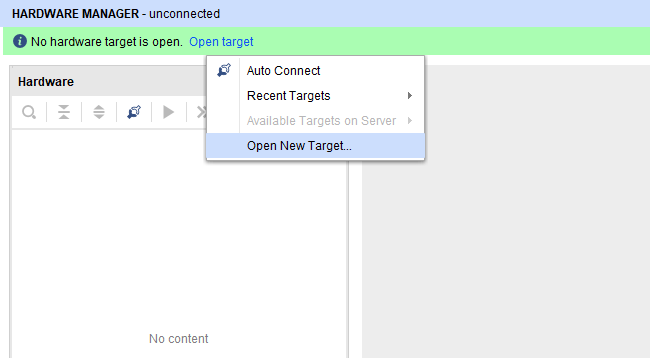
\includegraphics[scale=0.4]{image/l1_hard_1.png}   
			\label{l1_hard_1}
		\end{minipage}
	}
	\subfigure[Окно мастера подключения нового устройства] 
	{
		\begin{minipage}{8cm}
			\centering      
			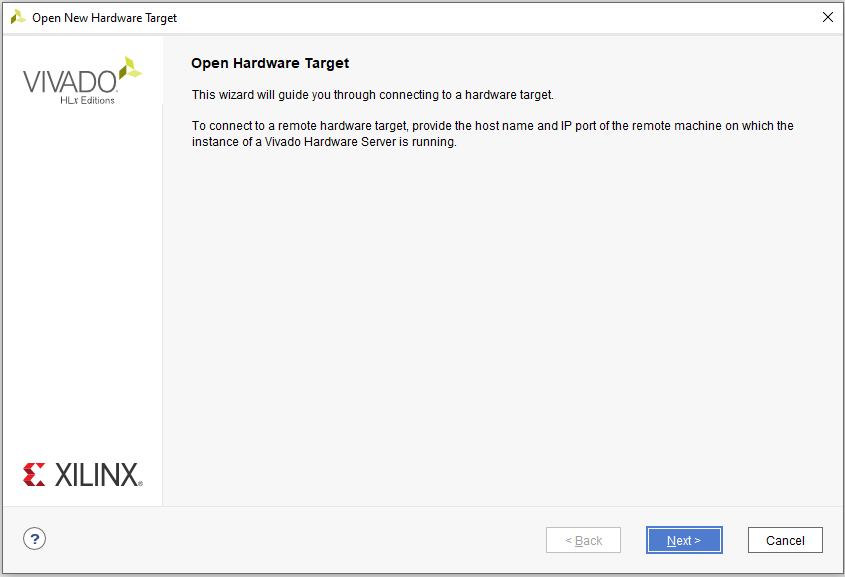
\includegraphics[scale=0.4]{image/l1_hard_2.png}   
			\label{l1_hard_2}
		\end{minipage}
	}
	\caption{Окно мастера подключения нового устройства: внешний вид} %  %Имя большого изображения
\end{figure}

\begin{figure}[htbp]	
	\subfigure[Hardware Server Setting] 
	{
		\begin{minipage}{9cm}
			\centering         
			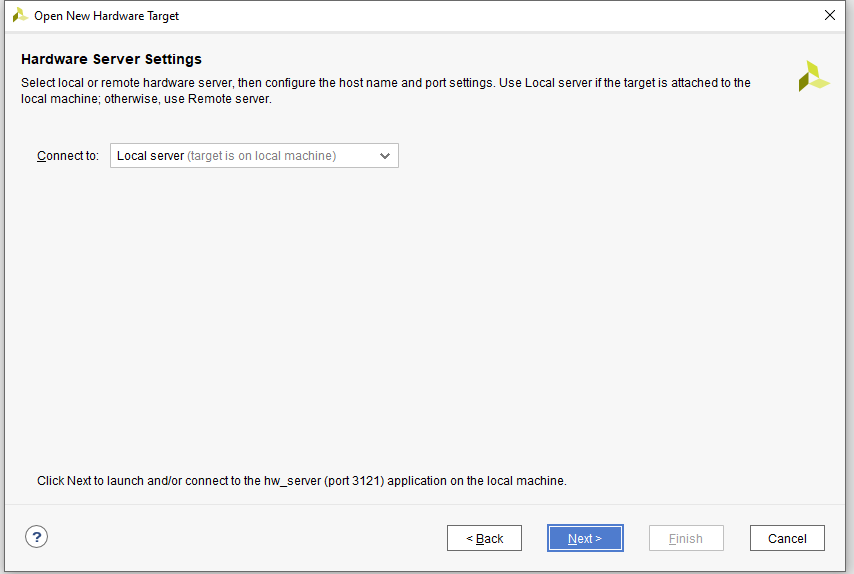
\includegraphics[scale=0.4]{image/l1_hard_3.png} 
			\label{l1_hard_3}
		\end{minipage}
	}
	\subfigure[Select Hardware Target] 
	{
		\begin{minipage}{9cm}
			\centering      
			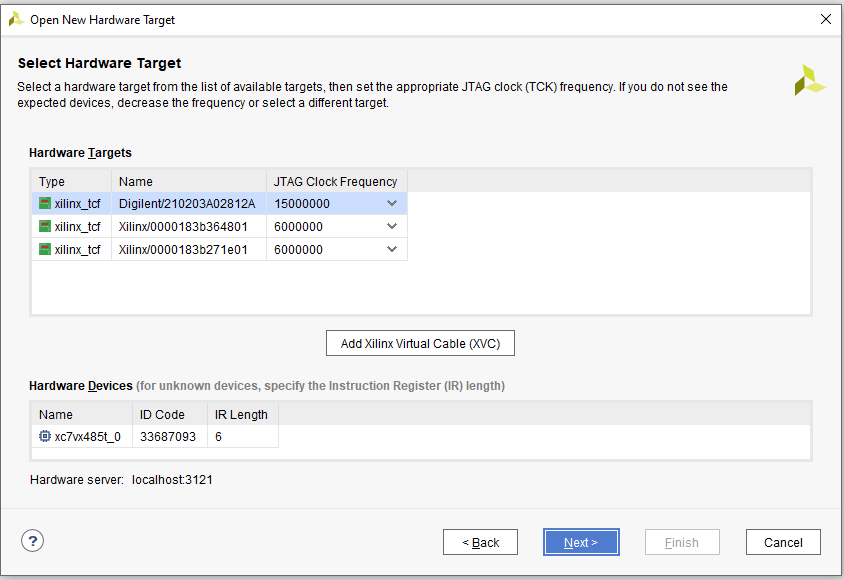
\includegraphics[scale=0.4]{image/l1_hard_4.png} 
			\label{l1_hard_4}
		\end{minipage}
	}
	\caption{Окно мастера подключения нового устройства: выбор устройства} %  %Имя большого изображения
\end{figure}

\begin{figure}[!ht]
	\centering
	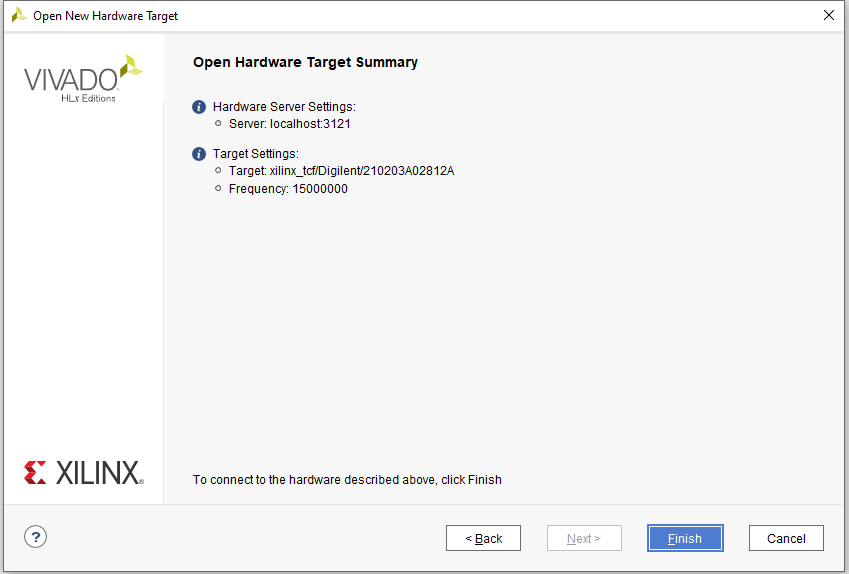
\includegraphics[width=0.5\textwidth]{image/l1_hard_sum.png}
	\caption{Окно мастера подключения нового устройства: результаты}
	\label{l1_hard_5}
\end{figure}

\begin{figure}[htbp]	
	\subfigure[Результаты подключения нового устройства] 
	{
		\begin{minipage}{8cm}
			\centering         
			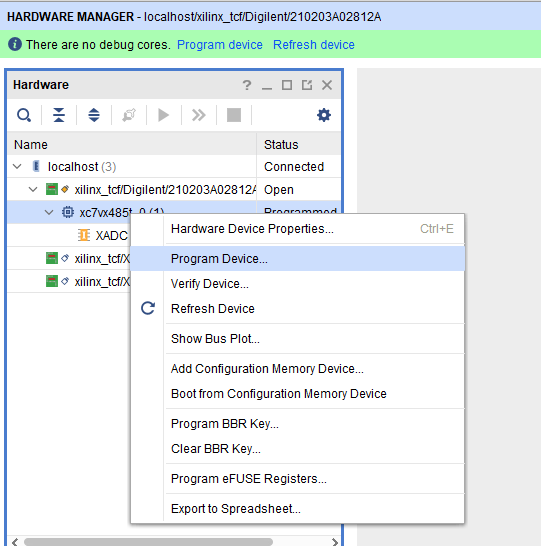
\includegraphics[scale=0.4]{image/program_0.png} 
			\label{l1_hard_6}
		\end{minipage}
	}
	\subfigure[Указываем путь к прошивке] 
	{
		\begin{minipage}{8cm}
			\centering      
			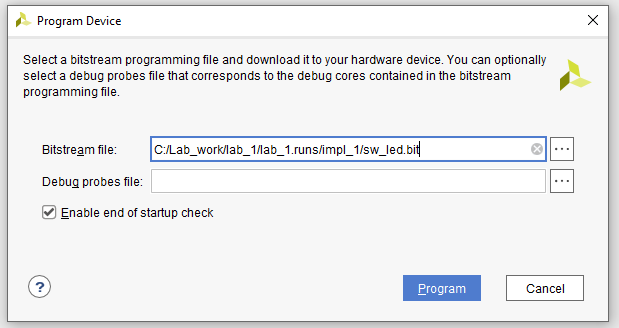
\includegraphics[scale=0.6]{image/program.png} 
			\label{l1_hard_7}
		\end{minipage}
	}
	\caption{Программирование ПЛИС} %  %Имя большого изображения
\end{figure}

\section{Иерархия проекта и простые логические элементы}

В проекте, особенно сложном, бывает много модулей, соединенных между собой. Прежде
всего, нужно заметить, что обычно в проекте всегда есть один модуль самого верхнего уровня
(top level). Внутри тела модуля верхнего уровня объявляються экземпляры других модулей и потом
соединяються друг с другом проводами. Рассмотрим как это делается на простейшом примере.

Логические модули И и И-НЕ можно описать на языке Verilog следующим образом: 

\begin{Verbatim}[tabsize=4]
module AND(output OUT, input IN1, input IN2);
 	assign OUT = IN1 & IN2;
endmodule
module NAND(output OUT, input IN1, input IN2);
 	assign OUT = ~(IN1 & IN2);
endmodule
\end{Verbatim}

Логические модули ИЛИ и ИЛИ-НЕ можно описать на языке Verilog следующим образом: 

\begin{Verbatim}[tabsize=4]
module OR(output OUT, input IN1, input IN2);
 	assign OUT = IN1 | IN2;
endmodule
module NOR(output OUT, input IN1, input IN2);
 	assign OUT = ~(IN1 | IN2);
endmodule
\end{Verbatim}

Логические модули Исключающее ИЛИ и Исключающее ИЛИ-НЕ, а также элемент НЕ 
можно описать на языке Verilog следующим образом: 

\begin{Verbatim}[tabsize=4]
module XOR(output OUT, input IN1, input IN2);
 	assign OUT = IN1 ^ IN2;
endmodule
module XNOR(output OUT, input IN1, input IN2);
 	assign OUT = ~(IN1 ^ IN2);
endmodule
module INV(output OUT, input IN);
 	assign OUT = ~IN;
endmodule
\end{Verbatim}

Итак, мы знаем про основные базовые логические элементы – и это тоже модули. Используем
их в модуле более высокого уровня. Сделаем однобитный сумматор по вот такой схеме: 

\begin{figure}[!ht]
	\centering
	
\includegraphics[width=0.7\textwidth]{image/Full_Adder.PNG}
	\caption{Полный сумматор на логических элементах}
	\label{full_adder}
\end{figure}

Этот сумматор складывает два однобитных числа a и b. При выполнении сложения однобитных
чисел может случиться «переполнение», то есть результат уже будет двухбитным (1+1=2 или в
двоичном виде 1’b1+1’b1=2’b10). Поэтому у нас есть выходной сигнал переноса \verb|c_out|.
Дополнительный входной сигнал \verb|c_in| служит для приема сигнала переноса от сумматоров
младших разрядов, при построении многобитных сумматоров.
Посмотрите, как можно описать эту схему на языке Verilog, устанавливая в теле модуля
экземпляры других модулей.

\begin{Verbatim}[tabsize=4]
module adder1 (
	output wire sum, 
	output wire c_out, 
	input wire a, 
	input wire b, 
	input wire c_in
); 
wire s1,s2,s3; 
AND and_inst_1
( 
	.OUT (s1), 
	.IN1 (a), 
	.IN2 (b) 
); 
XOR xor_inst_1
( 
	.OUT (s2), 
	.IN1 (a), 
	.IN2 (b) 
);
AND and_inst_2
( 
	.OUT (s3), 
	.IN1 (s2), 
	.IN2 (c_in) 
); 
OR or_inst
( 
	.OUT (c_out), 
	.IN1 (s1), 
	.IN2 (s3) 
); 
XOR xor_inst_3
(
	.OUT (c_out), 
	.IN1 (s2), 
	.IN2 (c_in)
);
endmodule
\end{Verbatim}

Порядок описания экземпляра модуля такой:

\begin{itemize}
    \item Пишем название модуля, тип которого нам нужен.
    \item Пишем название конкретно этого экземпляра модуля по шаблону  \verb|имя_inst|.
    \item Описываем подключения сигналов: точка и затем имя сигнала модуля, затем в скобках
имя проводника, который сюда подключен. 

\end{itemize}
 
Конечно, совсем не обязательо описывать наш модуль так, как описано выше. Честно говоря,
мне гораздо приятней видеть вот такой код однобитного сумматора: 

\begin{Verbatim}[tabsize=4]
module adder1(
	output wire sum, 
	output wire c_out, 
	input wire a, 
	input wire b, 
	input wire c_in
);
	assign sum = (a^b) ^ c_in;
	assign c_out = (a & b) |  (c_in & (a ^ b));
endmodule
\end{Verbatim}

Просто важно понимать, что существуют разные методы описания, и нужно уметь ими всеми
пользоваться.

\section{Мультиплексор и параметризация модуля}

Рассмотрим реализацию мультиплексора 2->1 на языке Verilog.

\begin{Verbatim}[tabsize=4]
module mux_2to1 ( 
	input wire a,                   
	input wire b,                                    
	input sel,               
	output out
);             
  
   assign out = sel ? b : a;  
  
endmodule  
\end{Verbatim}

Усложним задачу и построим мультиплексор 4->1. 

\begin{Verbatim}[tabsize=4]
module mux_4to1 ( 
	input wire a,                   
	input wire b,                   
	input wire c,                   
	input wire d,                   
	input [1:0] sel,               
	output out
);             
  
   assign out = sel[1] ? (sel[0] ? d : c) : (sel[0] ? b : a);  
  
endmodule  
\end{Verbatim}

Пусть теперь мы хотим коммутировать не просто провода, а шины, при этом нам нужно два мультиплексора под различные размеры шин. Пусть один мультиплексор коммутирует 8-битные шины, а другой 16-битные.
Тогда мы получим следующий код:

\begin{Verbatim}[tabsize=4]
module mux_4to1 ( 
	input wire [7:0] a,                   
	input wire [7:0] b,                   
	input wire [7:0] c,                   
	input wire [7:0] d,                   
	input [1:0] sel,               
	output [7:0] out
);             
  
   assign out = sel[1] ? (sel[0] ? d : c) : (sel[0] ? b : a);  
  
endmodule  
\end{Verbatim}

\begin{Verbatim}[tabsize=4]
module mux_4to1 ( 
	input wire [15:0] a,                   
	input wire [15:0] b,                   
	input wire [15:0] c,                   
	input wire [15:0] d,                   
	input [1:0] sel,               
	output [15:0] out
);             
  
   assign out = sel[1] ? (sel[0] ? d : c) : (sel[0] ? b : a);  
  
endmodule  
\end{Verbatim}

Эти модули не отличаются ни чем, кроме размера шин.
Используя параметризацию в языке Verilog можно построить мультиплексор с размером шины переменным(до синтеза), а не постоянным. Параметризованный модуль мультиплексора имеет следующий вид:

\begin{Verbatim}[tabsize=4]
module mux_4to1 #(
	parameter DATA_WIDTH = 8
) 
( 
	input wire [DATA_WIDTH - 1:0] a,                   
	input wire [DATA_WIDTH - 1:0] b,                   
	input wire [DATA_WIDTH - 1:0] c,                   
	input wire [DATA_WIDTH - 1:0] d,                   
	input [1:0] sel,               
	output [DATA_WIDTH - 1:0] out
);             
  
   assign out = sel[1] ? (sel[0] ? d : c) : (sel[0] ? b : a);  
  
endmodule  
\end{Verbatim}

При этом для подключения такого модуля используется следующий синтаксис:

\begin{Verbatim}[tabsize=4]
mux_4to1 #(
	.DATA_WIDTH(8)
)
mux_4to1_inst
( 
	.a(),                   
	.b(),                   
	.c(),                   
	.d(),                   
	.sel(),               
	.out()
);             
\end{Verbatim}

\newpage

Вопросы: 
\begin{enumerate}
\item Проведите функциональную симуляцию схемы по заданным входным сигналам a, b, clk.
\item 
\item 
\end{enumerate}

Задания:

\begin{enumerate}
	\item Реализовать модуль сумматора, используя простейшие логические элементы как отдельные модули, то есть необходимо получить проект с иерархией(см. подпункт. 1.2).
	\item Реализовать на языке Verilog следующие модули(число N узнать у преподавателя):
	\begin{enumerate}
		\item Шифратор (двоичный). На входе: \(2^N\)-битная маска вида 0010 (\verb|data_i|).
		На выходе: N-битное число, которое показывает номер бита, в котором выставлена единица (\verb|num_o|).
		
		\item Дешифратор (двоичный). На входе: N-битное число (\verb|num_i|). На выходе: \(2^N\) двоичная маска (\verb|dec_o|), 
		где стоит единица в бите под тем номером, который подан на вход.
		
		\item Мультиплексор. На входе: \(2^N\)-битные данные (\verb|data_i|), N-битный номер для выбора (\verb|num_i|).
		На выходе: значение бита, которой расположен под номером \verb|num_i|.

		\item Демультиплексор. На входе: один бит данных (\verb|data_i|), N-битный номер (\verb|num_i|).
		На выходе: данные размером \(2^N\) (\verb|data_o|), в бите под номером \verb|num_i| должно быть выставлено значение \verb|data_i|. Во всех остальных битах - нули.
	\end{enumerate}
	\item Реализовать на языке Verilog следующие логические функции:
	\begin{enumerate}
		\item (a XOR b) OR (c AND d)) AND (a AND b) OR (NOT c). 
		\item ((a OR d) AND (NOT c)) OR (d AND a) OR (c OR d) .
		\item (a AND b AND c ) OR ((c AND d) AND (c OR a)) OR (NOT d).
		\item (d XOR c) OR ((d XOR a) AND (c OR b)) AND (NOT a).
	\end{enumerate}
\end{enumerate}

\textbf{Для каждого представленного выше задания необходимо}:
\begin{enumerate}
\item Написать синтезируемый модуль, который решает поставленную задачу.
\item Написать модуль-тестбенч (testbench) к этому модулю.
\item Сделать проект в Vivado. Собрать модуль согласно заданию. 
\item Провести симуляцию в Vivado. Убедиться, что модуль корректно работает.
\item Написать файл ограничений для каждого проекта. Входы подключаем к кнопках, выходы к светодиодам.
\item Убедится, что модуль синтезируется, и не возникает латчей, комбинационных петель и пр.. Провести размещение и трассировку проекта, убедиться что нет ошибок. 
\item Сгенерировать конфигурационный файл, убедиться что успешно.
\end{enumerate}